% Credence Framework Tutorial
\documentclass[aspectratio=169]{beamer}

% Theme and packages
\usetheme{metropolis}
\usepackage[utf8]{inputenc}
\usepackage{amsmath, amssymb, mathtools, bm}
\usepackage{graphicx}
\usepackage{booktabs}
\usepackage{lmodern}
\usefonttheme{professionalfonts}
\usepackage{microtype}
\usepackage{xcolor}
\usepackage{hyperref}
\usepackage[absolute,overlay]{textpos}
\usepackage{tikz}
\usetikzlibrary{positioning,arrows.meta,shapes.geometric,calc}

\title[Credence]{Generating Semi-Synthetic Data for Causal Inference \\ \large The Credence Framework (\emph{Tutorial and app})}
\author{Andy Wilson\\
wilson.stats@gmail.com}
\institute{}
\date{}

\definecolor{accent}{HTML}{4A9EFF}
\setbeamercolor{structure}{fg=accent}
\setbeamercolor{background canvas}{bg=white}
\metroset{progressbar=frametitle,block=fill}
\setbeamertemplate{navigation symbols}{}
\setbeamertemplate{footline}{}

\newcounter{savedframenumber}

\begin{document}

% Title slide
\begin{frame}[plain]
  \titlepage
\end{frame}

% ----------------------------------------
\begin{frame}{The Validation Problem}
  \small
  When validating causal inference methods, we often use \textbf{simulated} data:
  \begin{itemize}
    \item Tools like \texttt{simcausal} generate data with known ground truth
    \item We can compare naive, G-computation, IPW, and TMLE estimates
    \item Methods can be evaluated against the true causal effect
  \end{itemize}
  \vspace{1em}

  \textbf{But how realistic is this synthetic data?}
  \begin{itemize}
    \item We hand-specify the DGP with parametric assumptions
    \item Real-world data has complex, non-linear relationships
    \item Would our estimator comparisons hold in messier settings?
  \end{itemize}
  \vspace{1em}

  \textcolor{accent}{\textbf{This tutorial:}} The \textbf{Credence framework} for generating more realistic synthetic data to validate causal methods
\end{frame}

% ----------------------------------------
\begin{frame}{The Estimator Choice Problem}
  \small
  \begin{columns}[T,totalwidth=\textwidth]
    \begin{column}{0.55\textwidth}
      Imagine you're a researcher familiar with causal methods.
      \begin{itemize}
        \item You face a choice among estimators: IPW, AIPW/DR/DML, TMLE, matching
        \item How do you know which works better on messy, confounded, finite-sample data?
        \item If you were like me, you'd simulate `realistic' data with \texttt{simcausal()}
        \item But even DAG-directed synthetic data lacks `gritty realism'
      \end{itemize}
    \end{column}
    \begin{column}{0.43\textwidth}
      \centering
      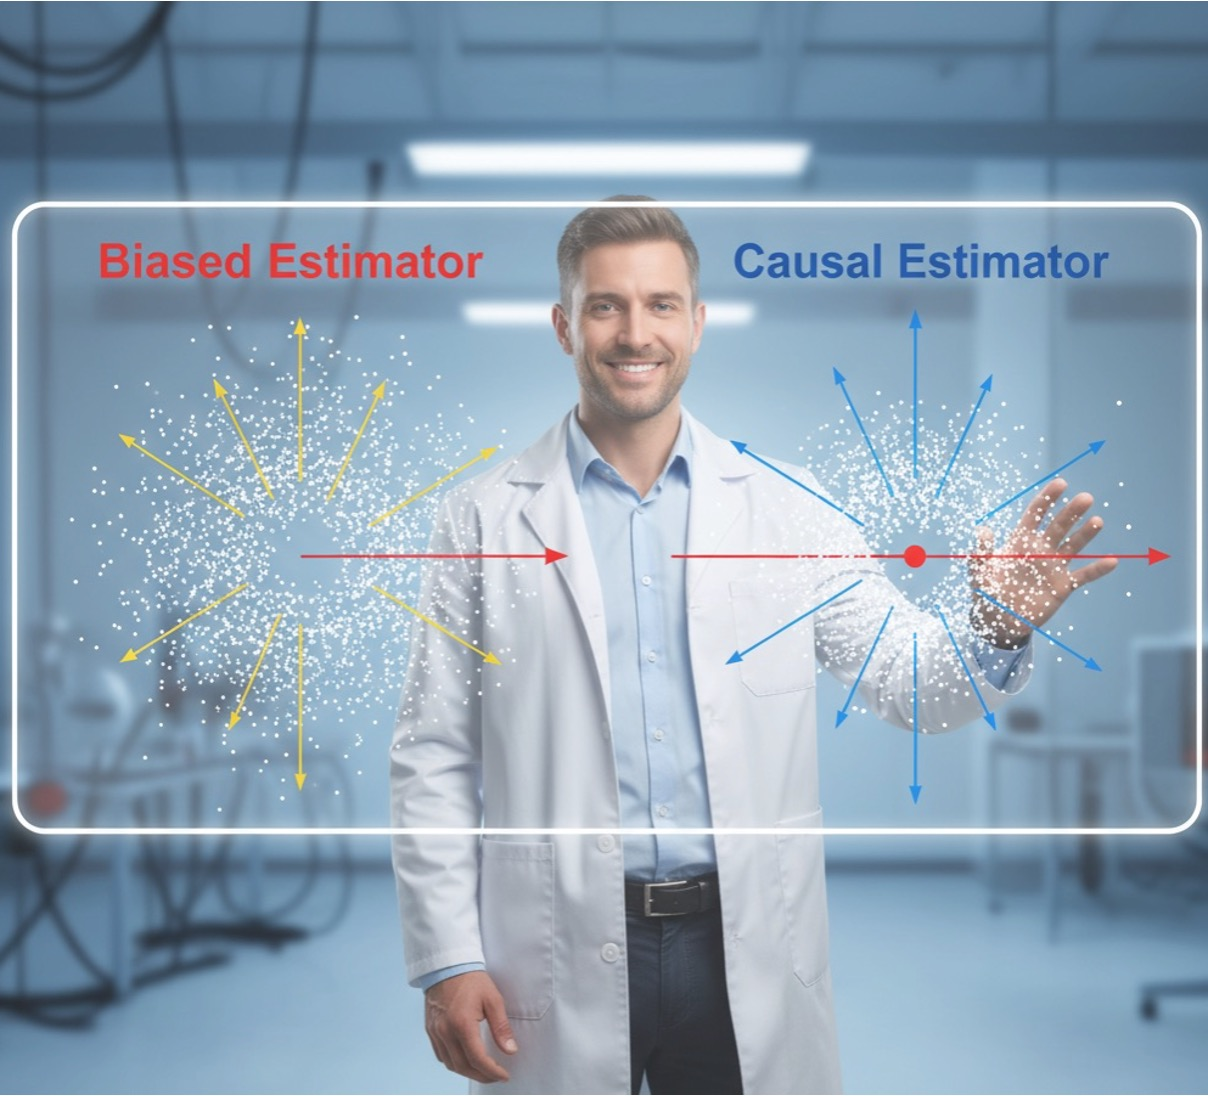
\includegraphics[width=0.9\linewidth]{images/Picture3.jpg}\\[0.5em]
      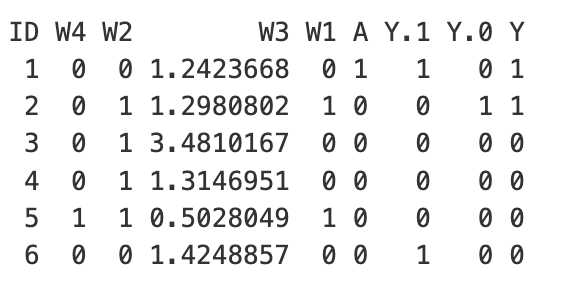
\includegraphics[width=0.9\linewidth]{images/simcausal3.png}
    \end{column}
  \end{columns}
\end{frame}

% ----------------------------------------
\begin{frame}{Left Wanting (my experience)}
  \small
  \begin{columns}[T,totalwidth=\textwidth]
    \begin{column}{0.5\textwidth}
      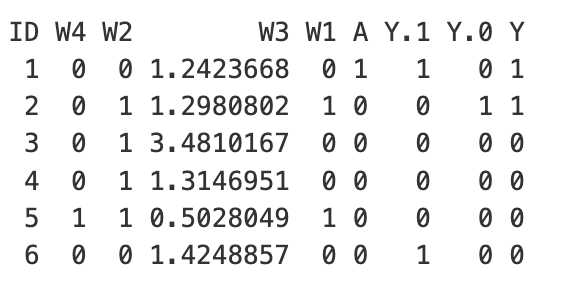
\includegraphics[width=\linewidth]{images/simcausal3.png}
    \end{column}
    \begin{column}{0.48\textwidth}
      \centering
      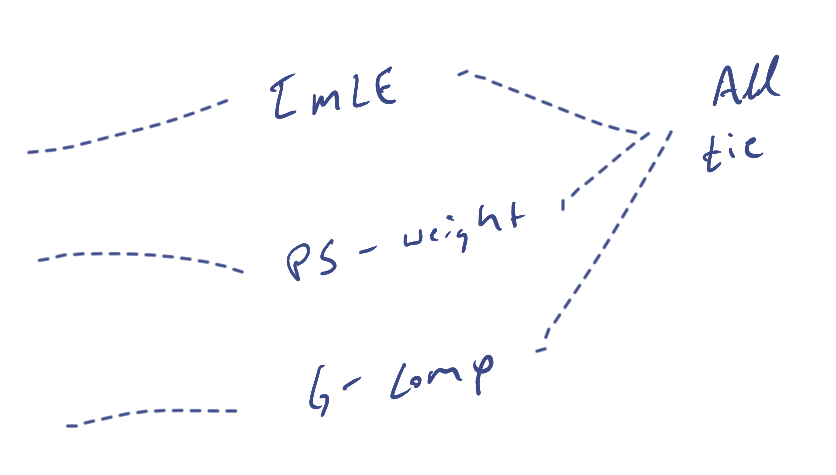
\includegraphics[width=\linewidth]{images/wanting.png}
    \end{column}
  \end{columns}
\end{frame}

% ----------------------------------------
\begin{frame}{Why Traditional Simulations Fall Short}
  \small
  How can we create data realistic enough to choose among estimators for \emph{real-world}, finite-sample settings?
  \begin{itemize}
    \item \textbf{Embedded assumptions:} stylized DGPs can privilege certain estimators
    \item \textbf{Simplifications:} MVN/DAG-only sims rarely match empirical $p(X)$ and $p(X\mid Z)$
    \item \textbf{Entanglement:} encoding truth often breaks empirical resemblance
    \item \textbf{Consequence:} misspecified DGPs and weak realism can mislead
  \end{itemize}
  \vspace{0.5em}
  \textbf{Goal:} Build semi-synthetic data with known ground truth on top of realistic structure $\rightarrow$ realism first, then controlled bias injection
\end{frame}

% ----------------------------------------
\begin{frame}{The Vision}
  \centering
  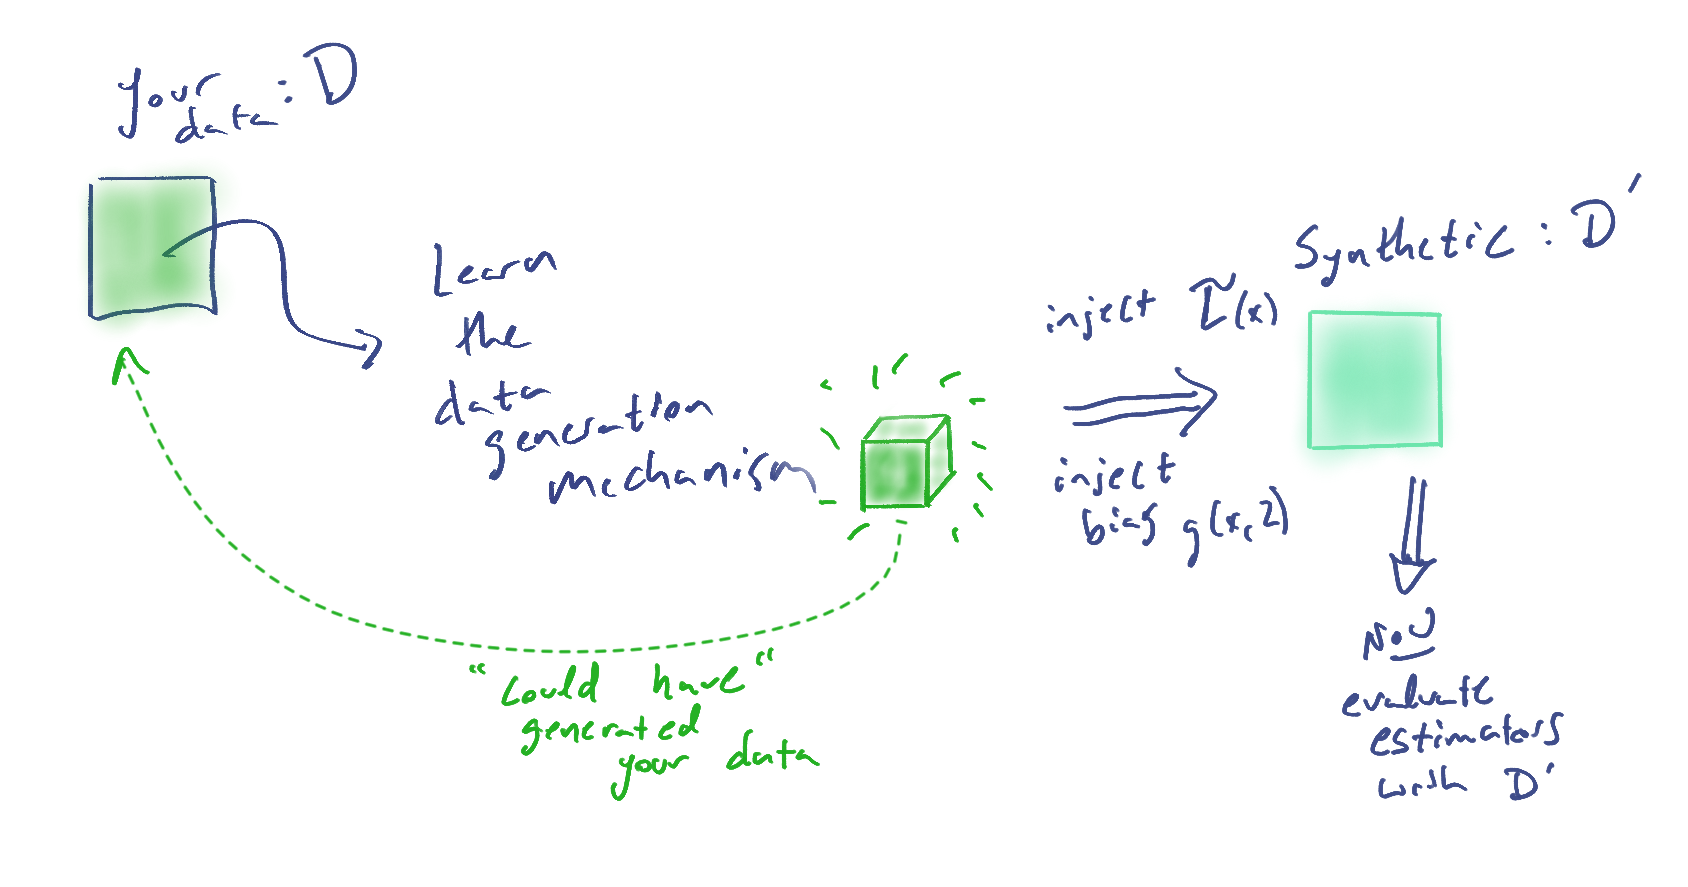
\includegraphics[width=0.8\linewidth]{images/Dream1.png}
\end{frame}

% ----------------------------------------
\begin{frame}{The Credence Framework}
  \small
  \centering
  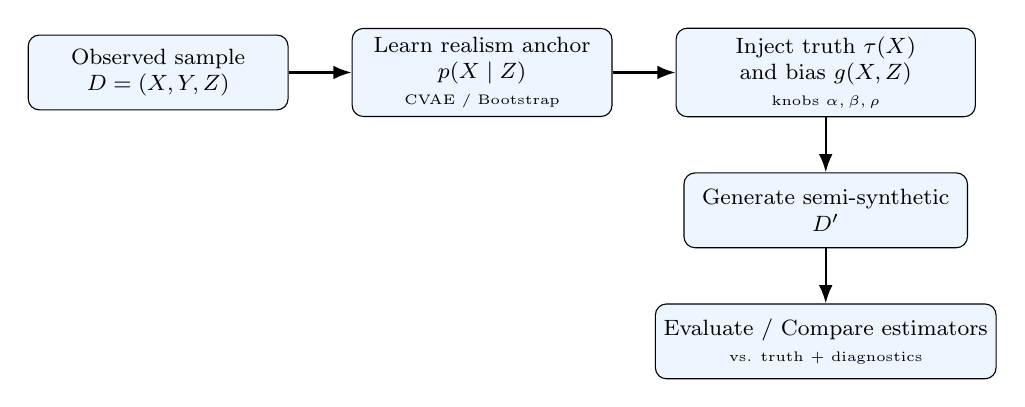
\begin{tikzpicture}[
    node distance=7mm and 8mm,
    >=Latex,
    box/.style={draw, rounded corners, fill=accent!10, inner sep=3pt, minimum width=3.3cm, minimum height=0.95cm, align=center},
    every node/.style={font=\footnotesize}
  ]
    % Top row
    \node[box] (obs) {Observed sample \\ $D=(X,Y,Z)$};
    \node[box, right=of obs] (learn) {Learn realism anchor \\ $p(X\mid Z)$ \\ {\tiny CVAE / Bootstrap}};
    \node[box, right=of learn, minimum width=3.8cm] (inject) {Inject truth $\tau(X)$ \\ and bias $g(X,Z)$ \\ {\tiny knobs $\alpha,\beta,\rho$}};
    % Downstream
    \node[box, below=of inject, minimum width=3.6cm] (gen) {Generate semi-synthetic \\ $D'$};
    \node[box, below=of gen, minimum width=3.8cm] (eval) {Evaluate / Compare estimators \\ {\tiny vs. truth + diagnostics}};
    % Arrows
    \draw[->, line width=0.8pt] (obs) -- (learn);
    \draw[->, line width=0.8pt] (learn) -- (inject);
    \draw[->, line width=0.8pt] (inject) -- (gen);
    \draw[->, line width=0.8pt] (gen) -- (eval);
  \end{tikzpicture}
  \\[0.25em]
  {\tiny  realism via $p(X\mid Z)$; inject target $\tau(X)$ and bias $g$ with rigidity $(\alpha,\beta)$; evaluate estimators under known truth.}
\end{frame}

% ----------------------------------------
\begin{frame}{Injecting Truth and Bias}
  \small
  \begin{itemize}
    \item Choose \(\tau(\mathbf X)\) (e.g., constant or heterogeneous).
    \item Hidden factor \(U\sim\mathcal N(0,1)\); baseline noise \(\varepsilon\sim\mathcal N(0,\sigma^2)\).
    \item Potential outcomes: \(Y(0)=h(X)+\gamma U+\varepsilon\), \(Y(1)=Y(0)+\tau(X)\).
    \item Treatment: \(\Pr(Z=1\mid U)=\mathrm{logit}^{-1}(\kappa+\rho U)\) to dial unobserved confounding (\(\kappa\): intercept; avoid clash with rigidity \(\alpha\)).
  \end{itemize}
\end{frame}

% ----------------------------------------
\begin{frame}{Credence Realism Pipeline}
  \small
  \begin{columns}[T,totalwidth=\textwidth]
    \begin{column}{0.52\textwidth}
      \textbf{Learning the realism anchor}
      \begin{enumerate}
        \item Preprocess once: fixed \texttt{model.matrix} for \(\mathbf X\); baseline $h(X)$ and propensity $\eta(X)$ for diagnostics.
        \item Train CVAE to model \(p(X\mid Z)\); encode $(X,Z)$, sample latent $U$, decode with $Z$ for realistic $X$.
      \end{enumerate}
      \vspace{0.4em}
      \small Conditional ELBO (Evidence Lower BOund) balances reconstruction fidelity with KL regularization; KL keeps the latent distribution near a simple prior so we can traverse and sample the learned manifold.
    \end{column}
    \begin{column}{0.45\textwidth}
      \textbf{Overlaying causal structure}
      \begin{itemize}
        \item Inject target truth $f(x)$ and bias $g(x,z)$ with rigidity $(\alpha,\beta)$.
        \item Bias knobs: hidden confounding $\rho$, positivity trimming, measurement noise.
        \item Compare estimators against known truth and share diagnostics/settings.
      \end{itemize}
    \end{column}
  \end{columns}
\end{frame}

% ----------------------------------------
\begin{frame}{The Credence Demo App}
  \small
  \textbf{Python Shiny app for hands-on exploration:}
  \begin{itemize}
    \item \textbf{Guided tutorial:} Walks through generating semi-synthetic data with controllable $\tau$ and $\rho$
    \item \textbf{Sandbox mode:} Experiment with alternative generators for $X \mid Z$ (Gaussian MVN, bootstrap)
    \item Same learn $\rightarrow$ generate $\rightarrow$ compare pipeline
  \end{itemize}
  \vspace{1em}

  \centering
  \textbf{Live app:}\\[0.5em]
  \url{https://andystats.shinyapps.io/causally-credible_tutorial/}
\end{frame}

% ----------------------------------------
\begin{frame}{Strawman Comparison: When Do Methods Agree?}
  \small
  Conditions under which PS-weighting, TMLE, and DML produce similar ATE:
  \begin{itemize}
    \item \textbf{Simple DGP:} additive/linear signal; weak interactions/nonlinearity.
    \item \textbf{Adequate overlap:} no extreme propensities; trim tails if needed.
    \item \textbf{Well-specified learners:} logistic PS and linear outcome work reasonably.
    \item \textbf{No hidden bias:} set \(\rho=0\); measurement error off.
  \end{itemize}
  \vspace{0.3em}
  Expectation: all consistent methods center near the true ATE; TMLE/DR/DML offer small robustness/CI advantages.
\end{frame}

% ----------------------------------------
%\begin{frame}[plain]
%  \begin{tikzpicture}[remember picture,overlay]
%    \node[opacity=0.14] at (current page.center){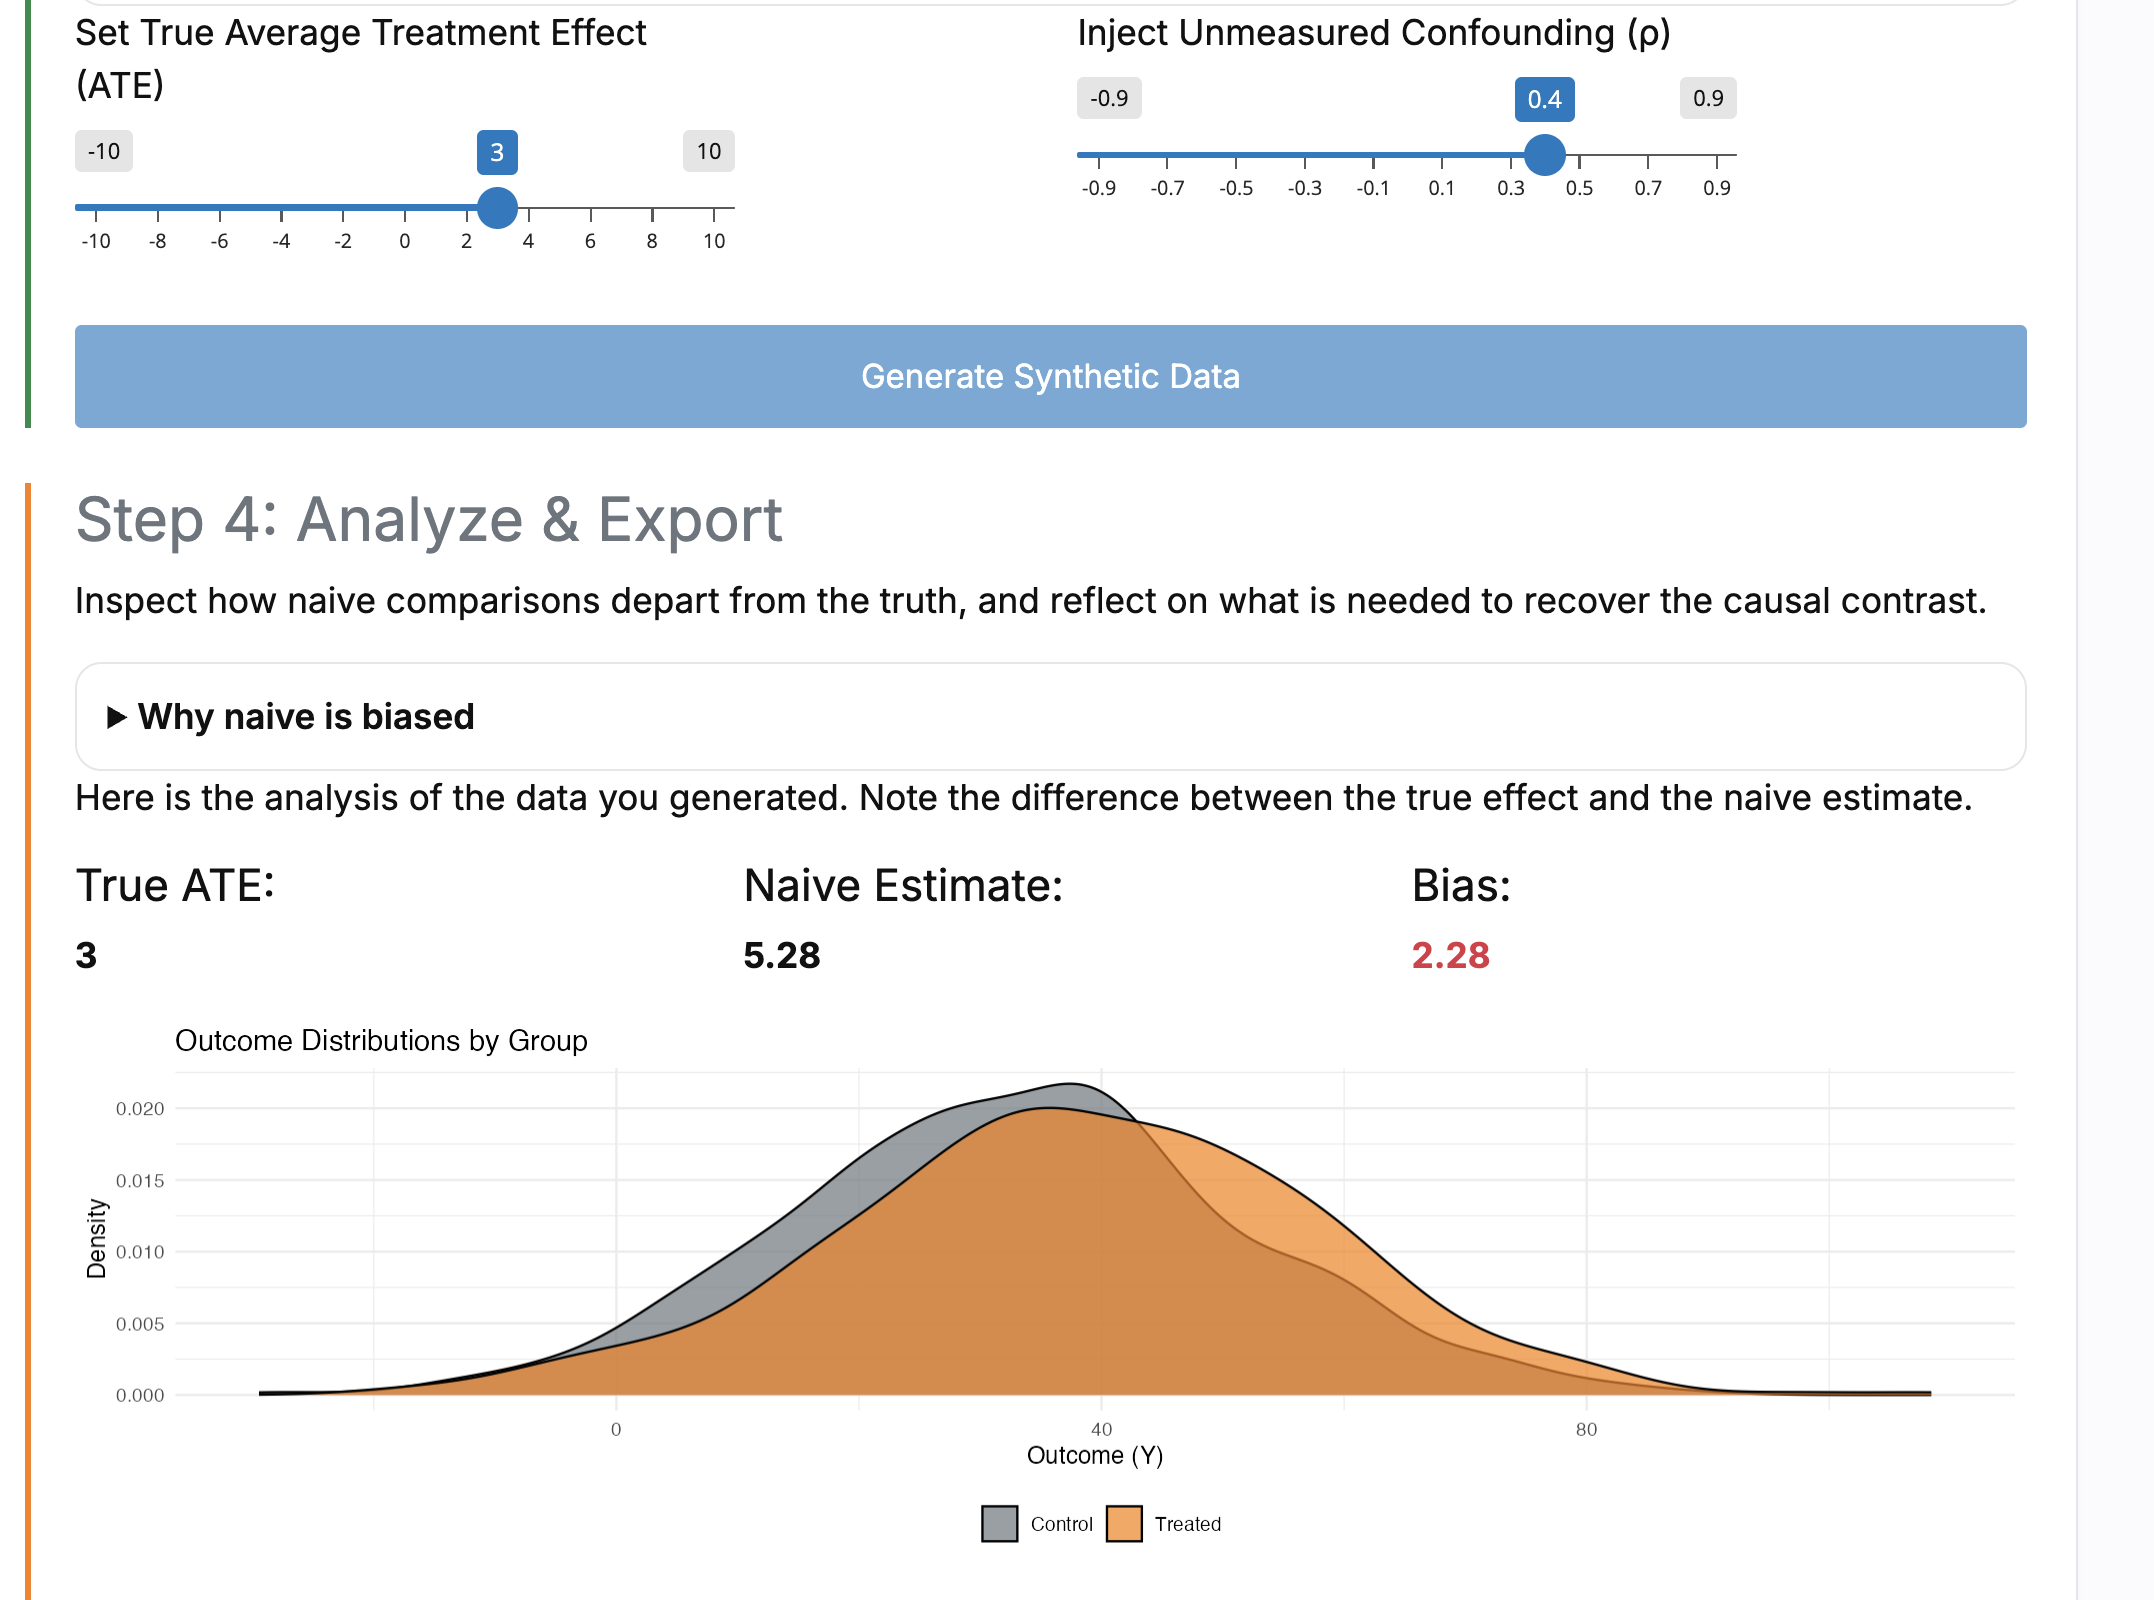
\includegraphics[width=0.70\paperwidth]{images/app.png}};
%  \end{tikzpicture}
 % \vfill
%  \centering
 % {\Huge Let's play}
%  \vfill
%\end{frame}

% ----------------------------------------
\begin{frame}{Summary and Applications}
  \small
  \textbf{Key takeaways:}
  \begin{itemize}
    \item Credence separates realism ($p(X\mid Z)$) from causal truth ($\tau(X)$)
    \item Pipeline: Learn $\rightarrow$ Inject $\tau$ and bias $\rightarrow$ Compare estimators
    \item CVAE provides flexible realism anchors; bias knobs ($\rho$, positivity) enable sensitivity analysis
  \end{itemize}
  \vspace{0.5em}

  \textbf{Applications:}
  \begin{itemize}
    \item \textbf{Method development:} Test estimators under realistic conditions
    \item \textbf{Sensitivity analysis:} Dial bias knobs to understand robustness
    \item \textbf{Education:} Show when methods agree vs. diverge
    \item \textbf{Regulatory:} Build credible validation datasets for real-world evidence
  \end{itemize}
\end{frame}

% ----------------------------------------
\begin{frame}{}
  \vfill
  \centering
  \Large
  \textbf{Questions?}

  \vspace{2em}

  \normalsize
  Try the app: \url{https://andystats.shinyapps.io/causally-credible_tutorial/}

  \vspace{1em}

  \small
  Code: \url{https://github.com/andystats/causally-credible}
  
    \vspace{1em}

  \small
  email: wilson.stats@gmail.com
  
  \vfill
\end{frame}

\setcounter{savedframenumber}{\value{framenumber}}
\appendix
\setcounter{framenumber}{\value{savedframenumber}}

% ----------------------------------------
\begin{frame}{[Optional] Credence framework (expanded)}
  \small
  \begin{itemize}
    \item  Make \(D'=(X',Y',Z')\) match \(D\); minimize distance \(d\big((X,Y,Z),(X',Y',Z')\big)\).
    \item \textbf{Constraints:} inject truth \(f(x)=\mathbb E[Y(1)-Y(0)\mid X=x]\) and bias \(g(x,z)\) with rigidity \((\alpha,\beta)\).
    \item \textbf{Bias knobs:} \(\rho\) (latent confounding) and overlap/positivity; others optional.
    \item \textbf{Learn realism:} fit \(P(X\mid Z)\) (CVAE or bootstrap); keep diagnostics lightweight.
    \item \textbf{Benchmark:} compare estimators against known truth and report settings.
  \end{itemize}
\end{frame}

% ----------------------------------------
\begin{frame}{Conditional VAE Schematic}
  \small
  \begin{columns}[T,totalwidth=\textwidth]
    \begin{column}{0.46\textwidth}
      \centering
      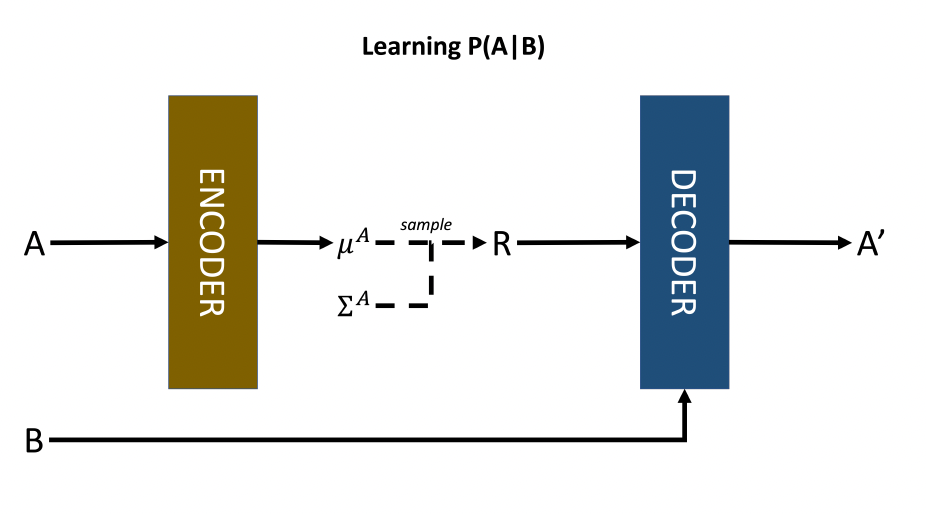
\includegraphics[width=0.95\linewidth]{images/figure2.png}
      \vspace{0.4em}
      {\tiny Adapted from Parikh et al. (2022).}
    \end{column}
    \begin{column}{0.52\textwidth}
      \footnotesize
      \textbf{Intuition.}
      \begin{itemize}
        \item Encoder compresses $(A,B)$ into a latent $U$ that keeps the signal needed to rebuild $A$.
        \item Decoder mixes $(U,B)$ to regenerate $A$; sampling $U$ yields draws from $P(A\mid B)$.
        \item KL regularization keeps $U$ near a simple prior so the model generalizes rather than memorizes.
      \end{itemize}
      \vspace{0.35em}
      \textbf{Why it matters here.}
      \begin{itemize}
        \item Realism knob: the CVAE learns the empirical $P(X\mid Z)$ so draws stay close to the observed covariates.
        \item Simulation knob: once trained, we can dial $Z$ and sample many $X$ quickly for Credence experiments.
      \end{itemize}
    \end{column}
\end{columns}
\end{frame}

% ----------------------------------------
\begin{frame}[plain]
  \begin{tikzpicture}[remember picture,overlay]
    \node[opacity=0.2] at (current page.center)
      {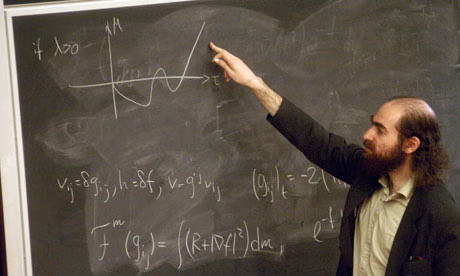
\includegraphics[height=\paperheight]{images/perelman.png}};
  \end{tikzpicture}
  \vfill
  \centering
  {\Large \textsc{Geometer's Corner}}\\[0.5em]
  {\small Latent manifolds, KL flows, and Credence knobs}
  \vfill
\end{frame}

% ----------------------------------------
\begin{frame}{Deep Dive: Framework (2.1) — Spaces (Figure)}
  \centering
  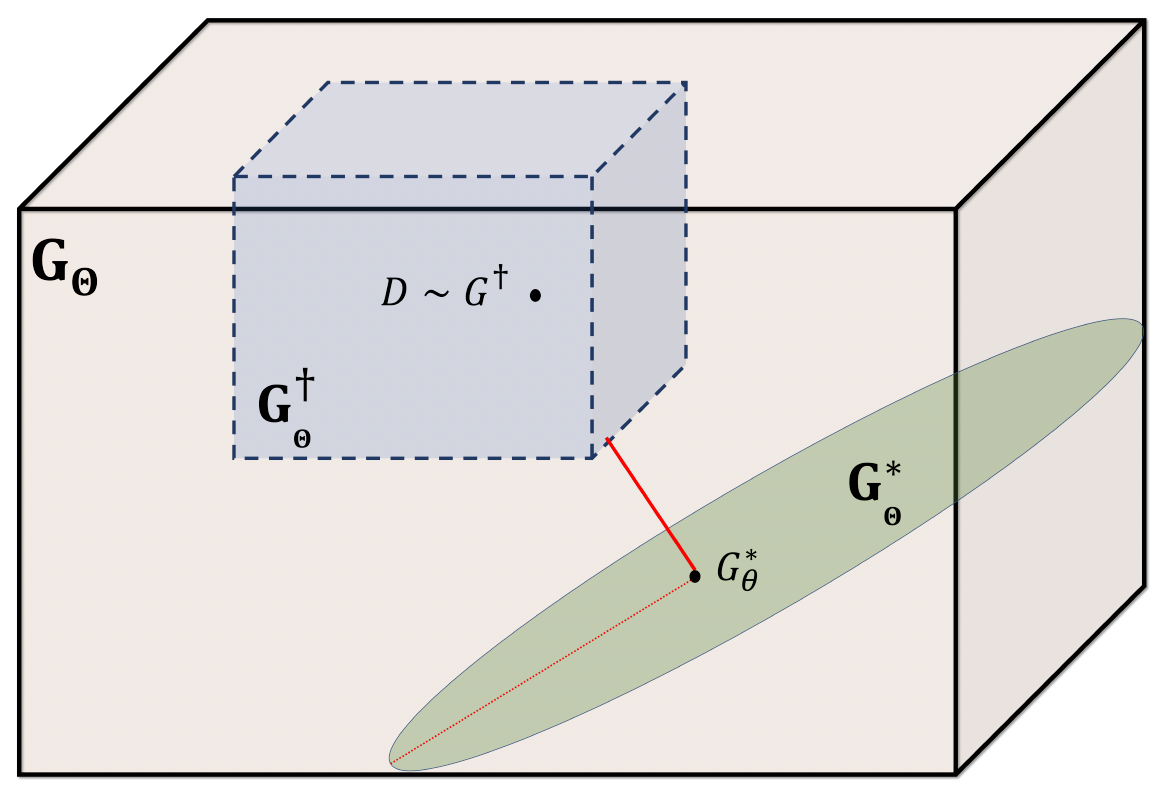
\includegraphics[width=8cm]{images/Figure1.png}
  \\[0.3em]
  {\tiny Figure 1 (Parikh et al. 2022): \(G_\Theta\), \(G^\dagger\), \(G^\dagger_\Theta\) (empirically isomorphic), \(G^*_\Theta\).\\
  Goal: find \(G^*_\theta\) in the overlap or closest under distance \(d\).}
\end{frame}

% ----------------------------------------
\begin{frame}{Objective as Tug-of-War}
  \small
  \centering
  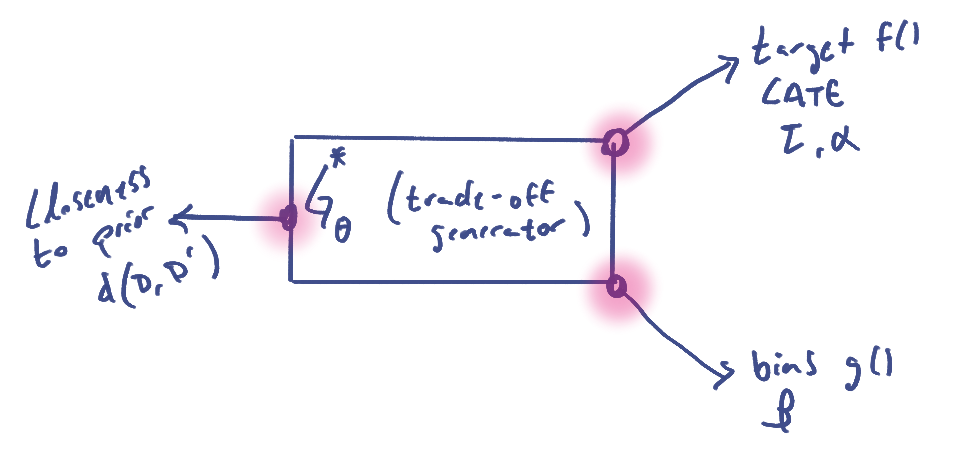
\includegraphics[width=0.65\linewidth]{images/tug_of_war.png}
  \vspace{0.3em}
  \begin{itemize}
    \item $d(D,D')$ keeps us glued to observed manifold; $\alpha$, $\beta$ pull toward causal knobs
    \item If $\alpha = \beta = 0$, we sit in $G^\dagger_\Theta \cap G^*_\Theta$ --- samples from empirical isomorphism
    \item KL-regularized learning explains why these forces don't tear realism apart
  \end{itemize}
\end{frame}

% ----------------------------------------
\begin{frame}{KL in the VAE Objective}
  \small
  \[
    \mathcal L = \underbrace{\mathbb E_{q_\phi(z\mid x)}\big[\log p_\theta(x\mid z)\big]}_{\text{reconstruction}} -
    \underbrace{D_{\mathrm{KL}}\!\big(q_\phi(z\mid x)\,\|\,p(z)\big)}_{\text{regularization}}
  \]
  \begin{itemize}
    \item Encoder $q_\phi(z\mid x)$ learns latent distributions; decoder $p_\theta(x\mid z)$ maps back
    \item KL keeps encoders near a simple prior ($\mathcal N(0,I)$), shaping a usable latent manifold
    \item In Credence this realism anchor lets us inject truth/bias without drifting from observed geometry
  \end{itemize}
\end{frame}

% ----------------------------------------
\begin{frame}{Geometric Intuition: KL as Prior Pull}
  \small
  \centering
  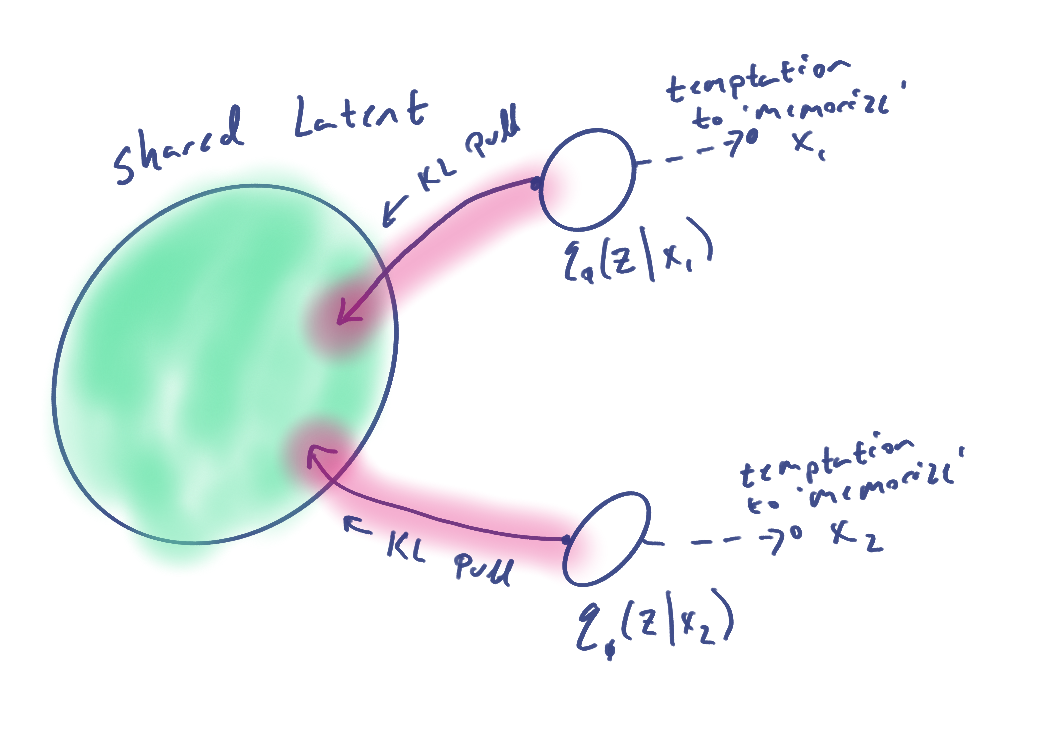
\includegraphics[width=0.48\linewidth]{images/KLpull.png}
  \vspace{0.6em}
  \footnotesize
  \begin{itemize}
    \item KL strength acts like an attraction to the shared manifold; weak KL lets posteriors drift into memorisation spikes.
    \item Balancing that attraction mirrors other manifold-regularised ideas (e.g., Aleph One); Credence taps the same geometry to stay realistic.
  \end{itemize}
\end{frame}

% ----------------------------------------
\begin{frame}{$\beta$-VAE: Tuning the Regularization}
  \small
  \begin{equation*}
    \mathcal L_\beta = \mathbb E_{q_\phi(z\mid x)}[\log p_\theta(x\mid z)] - \beta\, D_{\mathrm{KL}}\!\big(q_\phi(z\mid x)\,\|\,p(z)\big)
  \end{equation*}
  \vspace{0.4em}
  \begin{itemize}
    \item $\beta > 1$: stronger pull to the prior $\Rightarrow$ cleaner manifold, potential loss in reconstruction detail.
    \item $\beta < 1$: weaker pull $\Rightarrow$ sharper fits, risk of memorizing data and losing generative smoothness.
    \item Credence: treat VAE-$\beta$ as the latent-space sibling of $\alpha,\beta,\rho$; i.e., a knob that keeps realism and injected bias in balance.
  \end{itemize}
\end{frame}

% ----------------------------------------
\begin{frame}{Geometry Back to Credence}
  \small
  \begin{itemize}
    \item \textbf{Realism manifold:} KL-regularized CVAE shapes $p(X\mid Z)$ so \emph{`the vision'} sits on a learnable surface.
    \item \textbf{Knob legitimacy:} $d$, $\alpha$, $\beta$, $\rho$, and VAE-$\beta$ become coordinated forces, each with a geometric role.
    \item \textbf{Estimator insight:} when performance shifts we know if realism, truth, or bias pulled the generator off balance.
    \item \textbf{Full circle:} The geometry explains why Credence's knobs deliver the benchmarking datasets we wanted (and we can trust the process).
  \end{itemize}
\end{frame}

% ----------------------------------------
\begin{frame}{References}
  \footnotesize
  \textbf{Credence Framework:}
  \begin{itemize}
    \item Parikh H, et al.\ (2022). Validating Causal Inference Methods. \textit{ICML}. arXiv:2202.04208
  \end{itemize}

  \textbf{Related Methods:}
  \begin{itemize}
    \item Kingma \& Welling (2014). Auto-Encoding Variational Bayes. \textit{ICLR}.
    \item Higgins et al.\ (2017). $\beta$-VAE. \textit{ICLR}.
  \end{itemize}

  \textbf{Software:}
  \begin{itemize}
    \item Credence App: \url{https://andystats.shinyapps.io/causally-credible_tutorial/}
    \item \texttt{simcausal} R package
  \end{itemize}
\end{frame}

\end{document}
